\documentclass[a4paper,12 pt]{article}
\usepackage[T2A]{fontenc}
\usepackage[utf8]{inputenc}
\usepackage[english, russian]{babel}
\usepackage{geometry}
\usepackage{float}
 \geometry{
 a4paper,
 top=25mm,
 }
\usepackage{amsmath, amsfonts, amssymb, amsthm, mathtools, indentfirst, float, wrapfig}
\usepackage{graphicx}
\begin{document}
    \begin{titlepage}
    \begin{center}
        \vspace{4cm}
        \huge {\textbf{Отчет о выполнении лабораторной работы 1.4.2 }}
        {} \\
        \vspace{1cm}
        \Large {\textbf{Определение ускорения свободного падения}} \\
        \Large {\textbf{при помощи оборотного маятника}} \\
        \vspace{10cm}
        \begin{flushright}
        \begin{minipage}{.45\textwidth}
        \normalsize{\textbf{Студент:} Копытова Виктория Сергеевна}\\
        \textbf{Группа:} Б03-304\\
        \end{minipage}
        \end{flushright}   
    \end{center}
    \end{titlepage}
\newpage
 
\section{Аннотация}
\textbf{Цель работы:} с помощью оборотного маятника измерить величину ускорения сво-
бодного падения.
	
\textbf{В работе используются:} оборотный маятник с двумя подвесными призмами и
двумя грузами (чечевицами); электронный счётчик времени и числа колебаний;
подставка с острием для определения положения центра масс маятника; закреплённая на стене консоль для подвешивания маятника; металлические линейки, штангенциркуль длиной 1 м.

\section{Теоретические сведения}

Физическим маятником называют твёрдое тело, способное совершать
колебания в вертикальной плоскости, будучи подвешено за одну из своих
точек в поле тяжести. Ось, проходящая через точку подвес перпендикулярно плоскости качания, называется осью качания маятника.
При малых колебаниях период колебаний физического маятника определяется формулой
\begin{equation}
    T=2\pi \sqrt{\frac{I}{gml}},
\end{equation}

где $I$ -- момент инерции маятника относительно оси качания, $m$ -- масса
маятника, $l$ -- расстояние от оси качания до центра масс маятника.
Если сравнить (1) с известной формулой колебаний математического
маятника длиной $l$ ($T = 2\pi \sqrt{l / g}$), можно определить приведённую длину
физического маятника как
\begin{equation}
    l_{\text{пр}} = \frac{I}{ml}.
\end{equation}
Смысл приведённой длины в том, что при длине математического маятника, равной $l_{\text{пр}}$, его период колебаний совпадает с периодом колебаний
физического маятника.

\textbf{Теорема Гюйгенса об оборотном маятнике}
\begin{figure}[H]
    \centering
    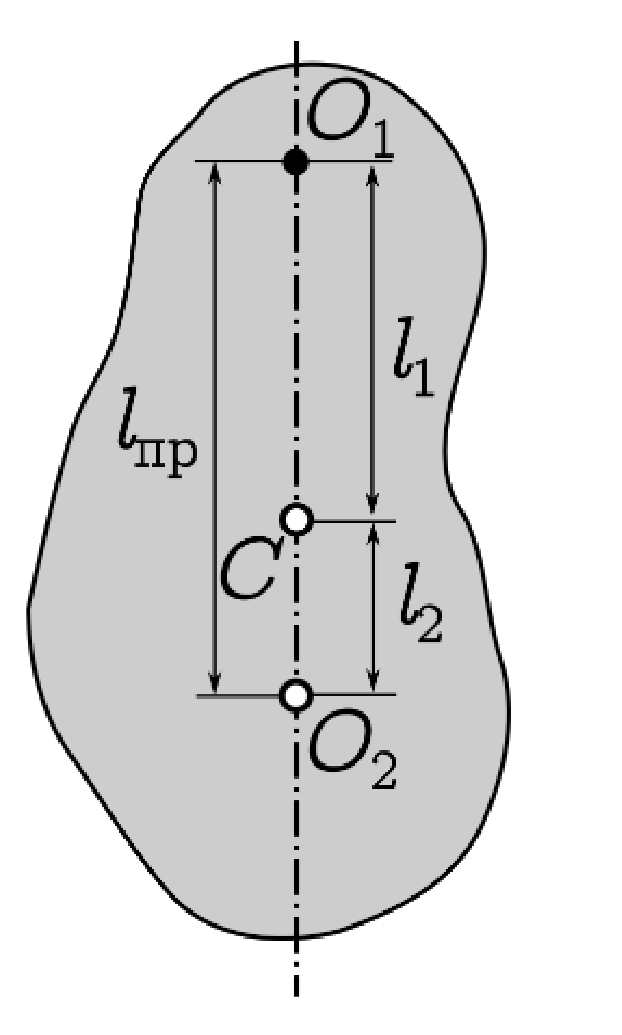
\includegraphics[scale = 0.3]{гюйгенс.png}
    \caption{К теореме Гюйгенса}
\end{figure}
Пусть $O_1$ — точка подвеса физического маятника, а
$C$ — его центр масс. Отложим отрезок длиной $l_{\text{пр}}$ вдоль
линии $O_1 C$, и обозначим соответствующую точку как $O_2$. Тогда
\begin{equation}
    T_1 = 2\pi \sqrt{\frac{I_1}{mgl_1}}, \quad T_2 = 2\pi \sqrt{\frac{I_2}{mgl_2}}.
\end{equation}

По теореме Гюйгенса—Штейнера имеем
\begin{equation}
    I_1=I_C + ml_1^2, \quad I_2=I_C + ml_2^2,
\end{equation}
где $I_C$ — момент инерции маятника относительно оси, проходящей через
центр масс перпендикулярно плоскости качания.
Пусть периоды колебаний одинаковы: $T_1$ = $T_2$ . Тогда одинаковы
должны быть и приведённые длины. C учётом (4) имеем
\begin{equation}
    l_{\text{пр}} = \frac{I_C}{ml_1} + l_1 = \frac{I_C}{ml_2} + l_2
\end{equation}
откуда следует, что при $l_1 \neq l_2$ справедливо равенство
\begin{equation}
    I_C = ml_1 l_2.
\end{equation}
Из (6) и (5) получим
\begin{equation}
    l_{\text{пр}} = l_1 + l_2.
\end{equation}

\textbf{Расчёт ускорения свободного падения}

Пусть $L = O_1 O_2 = l_1+l_2$ -- расстояние между двумя «сопряжёнными»
точками подвеса физического маятника. Если соответствующие периоды
малых колебаний равны, $T_1=T_2=T$, то по теореме Гюйгенса $L=l_{\text{пр}}$. Тогда из (1) и (2) находим ускорение свободного падения:
\begin{equation}
    g = (2\pi)^2 \frac{L}{T^2}
\end{equation}

Так как периоды не совпадают в точности, из (3) и (4) получаем
\begin{equation}
    g = (2\pi)^2 \frac{l_1^2-l_2^2}{T_1^2l_1-T_2^2l_2},
\end{equation}
что можно записать как
\begin{equation}
    g = g_0 \frac{\lambda-1}{\lambda - \frac{T_2^2}{T_1^2}},
\end{equation}
где $g_0 = (2 \pi)^2 L/T^2$, $\lambda=l_1/l_2$

Оценим добавку
\begin{displaymath}
    g = g_0 \frac{\lambda-1}{\lambda-(1+\varepsilon)^2} \approx g_0 \frac{\lambda}{\lambda-\frac{2\varepsilon}{\lambda-1}} \approx g_0 (1+2\beta \varepsilon),
\end{displaymath}
где $\varepsilon = \frac{\delta T}{T}$, $\beta = \frac{1}{\lambda-1} = \frac{l_2}{l_1-l_2}$.

Поэтому для большей точности опыта необходимо, чтобы выполнялось соотношение
\begin{displaymath}
    l_1>2,5l_2.
\end{displaymath}

\textbf{Оценка поггрешностей}
\begin{displaymath}
    \frac{\sigma_{g_0}}{g_0} = \sqrt{\Bigr(\frac{\sigma_L}{L} \Bigl) ^2 + 4 \Bigr(\frac{\sigma_T}{T} \Bigl) ^2}
\end{displaymath}
\begin{displaymath}
    g=g_0 + \Delta g, \quad \Delta g \approx \frac{2l_2}{l_1-l_2} \frac{\Delta T}{T} g_0
\end{displaymath}

Тогда 
\begin{displaymath}
    \frac{\sigma_{g}}{g} = \sqrt{\Bigr(\frac{\sigma_L}{L} \Bigl) ^2 + 4 \Bigr(\frac{\sigma_T}{T} \Bigl) ^2 + 8 \Bigr(\beta \frac{\sigma_T}{T} \Bigl) ^2 + 8 \Bigr(\beta \frac{\Delta T}{T} \frac{\sigma_l}{\Delta l} \Bigl) ^2}
\end{displaymath}

\textbf{Экспериментальная установка}

Применяемый в работе маятник представляет собой стержени цилиндрического сечения. Маятник подвешивается с помощью небольших треугольных призм ($ \text{П}_1, \text{П}_2$), острым основанием опирающихся на закреплённую на стене консоль. Ребро призмы задаёт ось качания маятника. На стержне закрепляются два дополнительных груза в форме «чечевицы» ($\text{Г}_1, \text{Г}_2$). Регистрация времени колебаний проводится с помощью электронных
счётчиков. Расстояния между точками установки маятников на консоли до
электронных счётчиков фиксировано.
\begin{figure}[H]
    \centering
    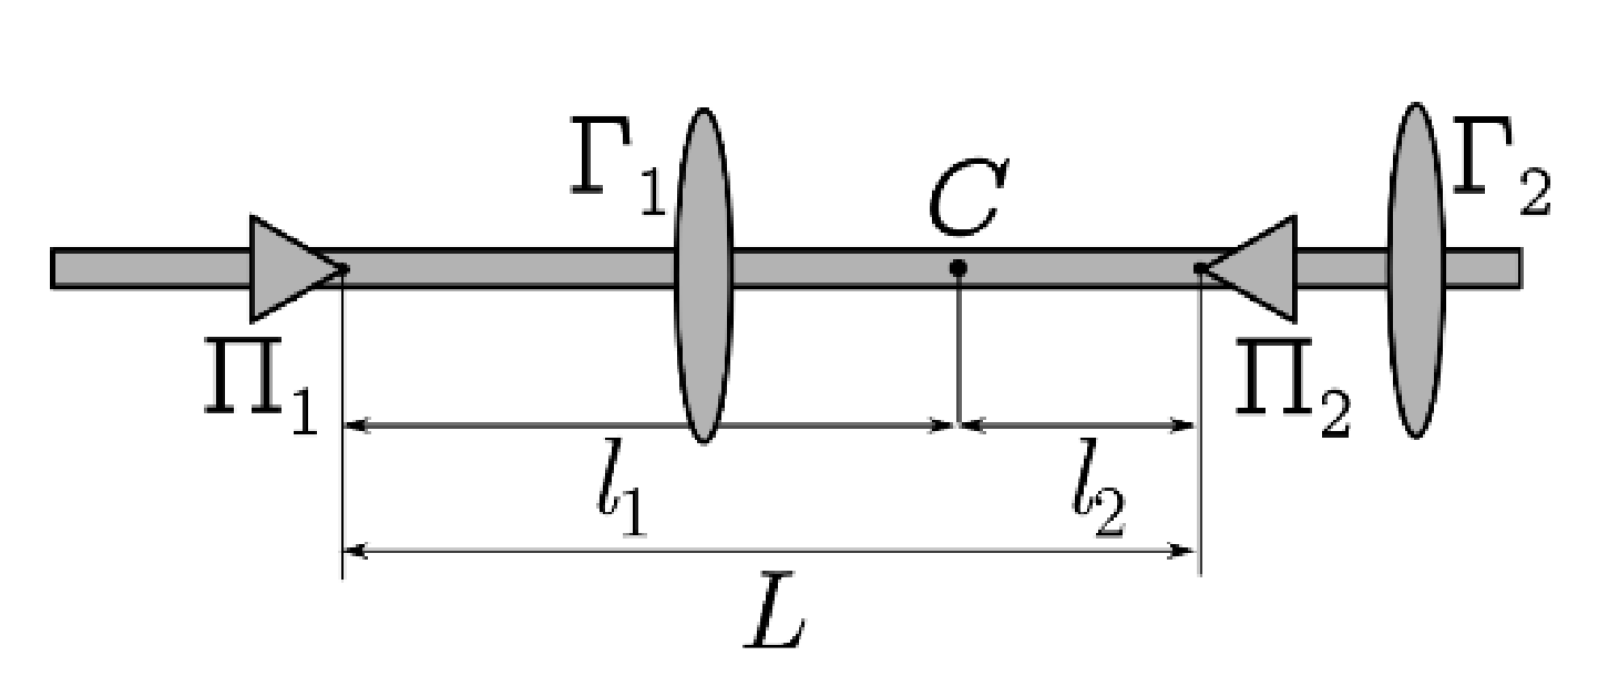
\includegraphics[scale=0.3]{маятник.png}
    \caption{Обороотный маятник}
\end{figure}



\section{Ход работы}

\begin{enumerate}
    \item Проведём измерение массы маятника целиком и всех его элементов по отдельности с помощью электронных весов. 
    \begin{table}[H]
        \centering
        \begin{tabular}{|c|c|}
            \hline
            Тело & Масса, г \\
            \hline
            Маятник & 4017,8 \\
            \hline
            Стержень & 868,3 \\
            \hline
            Призма $\text{П}_1$ & 78,3 \\
            \hline
            Призма $\text{П}_2$ & 79,6 \\
            \hline
            Груз $\text{Г}_1$ & 1471,5 \\
            \hline
            Груз $\text{Г}_2$ & 1495,7 \\
            \hline
        \end{tabular}
        \caption{Массы маятника и его составляющих}
    \end{table}
    \item Закрепим призмы 1 и 2 на стержне симмтерично дург относительно друга и измерим расстояние $L$ между призмами с помощью штангенциркуля.
    \begin{displaymath}
        L = (49,00 \pm 0,01) \text{см}.
    \end{displaymath}

    В дальнейшем призмы остаются закреплёнными на своих местах.
    \item Зададим соотношение $l_1/l_2 = 2,6$. Расчитаем положение грузов при котором периоды колебаний маятника при подвесе на призмы 1 и 2 будут одинаковыми.
    \begin{figure}[H]
        \centering
        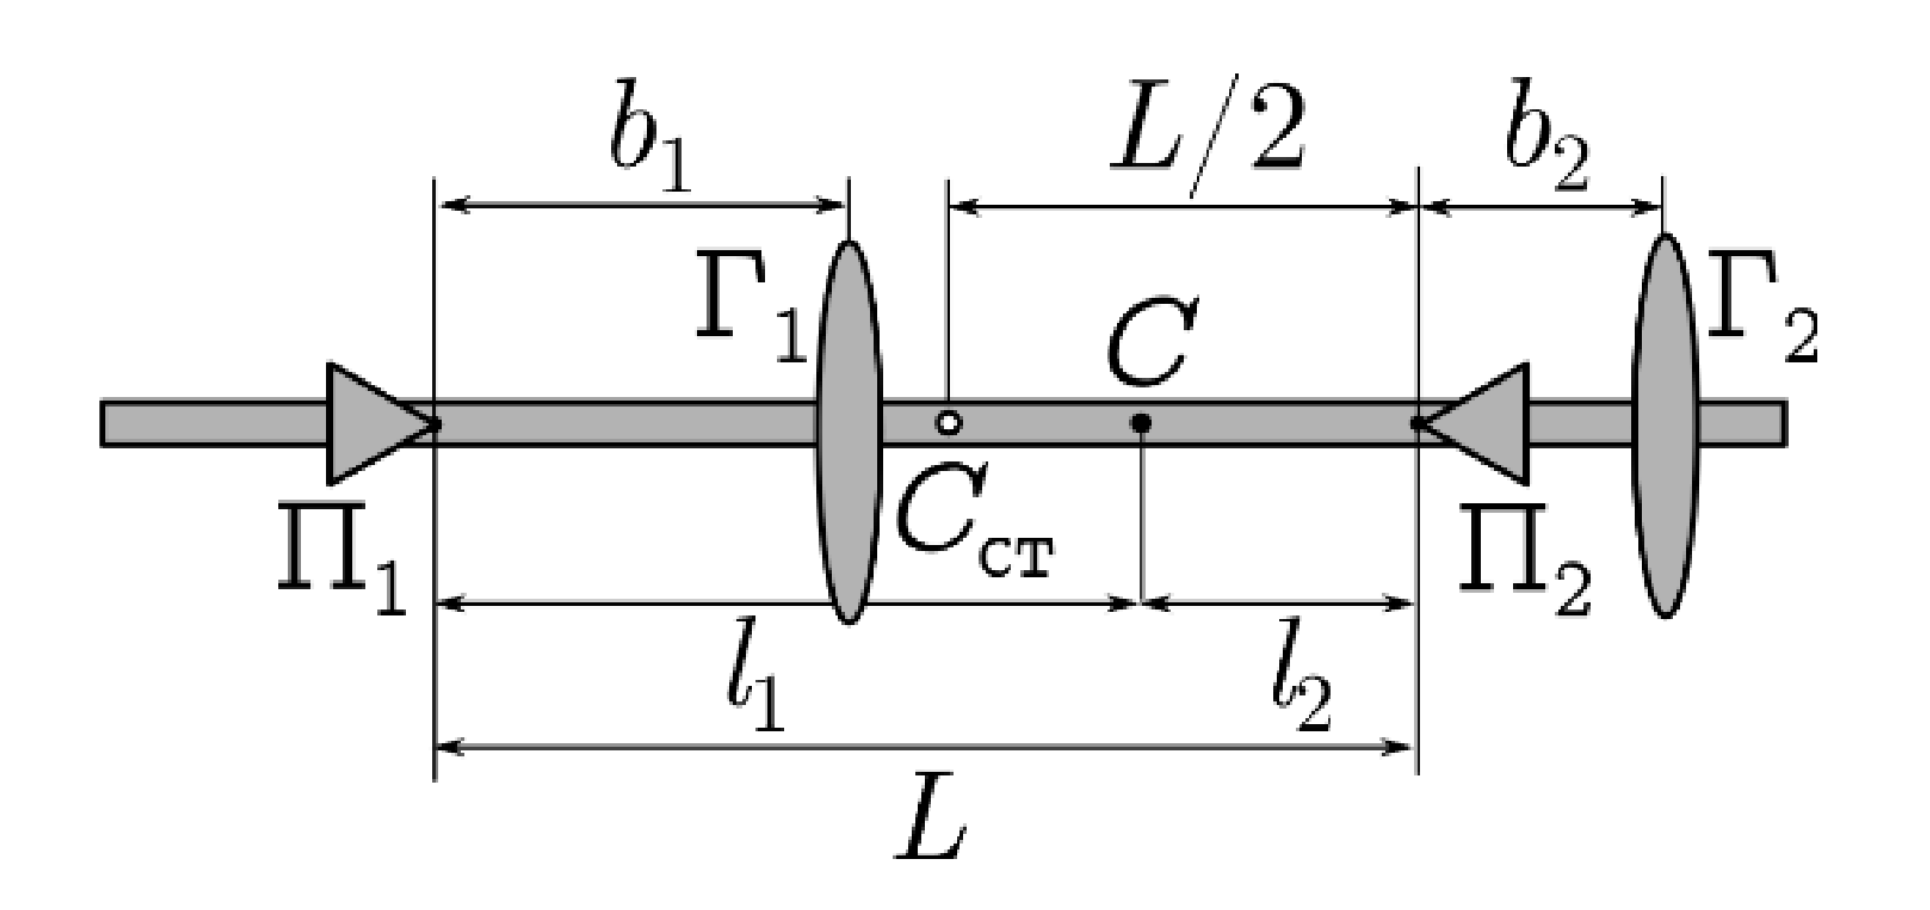
\includegraphics[scale = 0.3]{b}
        \caption{Оборотный маятник}
    \end{figure}
    Получаем 
    \begin{displaymath}
        b_1 = 20,9 \quad \text{см}
    \end{displaymath}
    \begin{displaymath}
        b_2 = 8,7 \quad \text{см}
    \end{displaymath}
    \item Определим положение центра масс маятника с грузами и с помощью этого значения определим $l_1$ и $l_2$.
    \begin{displaymath}
        l_1 = 34,8 \quad \text{см}
    \end{displaymath}
    \begin{displaymath}
        l_2 = 14,2 \quad \text{см}
    \end{displaymath}
    \item Проверим, что периоды колебаний маятника на призмах 1 и 2 достаточно точно совпадают.

    Среднее значение периода для призмы 1 
    \begin{displaymath}
        T_1 = 1,449 \quad \text{c}
    \end{displaymath}
    Среднее значение периода для призмы 2 
    \begin{displaymath}
        T_1 = 1,447 \quad \text{c}
    \end{displaymath}
    \begin{displaymath}
        \frac{\Delta T}{T} \approx 0,1 \%
    \end{displaymath}
    Периоды совпадают с достаточной для проведения эксперимента точностью.
    \item Проведём окончатеельное измерение периодов с максимальной точностью. Количество колебаний -- 150. Значения периодов
    \begin{displaymath}
        T_1 = 1,402 \quad \text{c}, \quad T_2 = 1,389 \quad \text{c}.
    \end{displaymath}
    \item Расчитаем ускорение свободного падения по формуле (9)
    \begin{displaymath}
        g = (2\pi)^2 \frac{l_1^2-l_2^2}{T_1^2l_1-T_2^2l_2} \approx 9.72 \quad \frac{\text{м}}{\text{c}^2}
    \end{displaymath}
    Погрешность $\sigma_g = 0,2 \quad \text{м} / \text{c}^2$

    Окончательный результат 
    \begin{displaymath}
        g = ( 9,72 \pm 0,2 ) \quad \text{м} / \text{c}^2
    \end{displaymath}

    Табличное значение ускорения свободного падения для Москвы $g_{\text{м}} = 9,815 \quad \text{м} / \text{c}^2$.

    Полученное значение совпадает с теоретическим в пределах погрешности. 
\end{enumerate}

\section{Вывод}

В ходе работы было измерено ускорение свободного падения. Результат измерения совпадает с табличным в пределах погрешности. Эта погрешность возникает из-за того, что не достигается точного совпадения периодов колебаний маятника для призм 1 и 2.

\end{document}


